L'algorithme de Dijkstra est un parcours en largeur d'un graphe \textbf{pondéré} et orienté. Il permet de calculer l'ensemble des plus courts chemins entre un sommet vers tous les autres sommets du graphe.

Pour modéliser le graphe, on utilisera une matrice d'adjacence $M$ pour laquelle $M_{ij}=w(i,j)$ et $w(i,j)$ représente le poids de l'arête de $i$ vers $j$. Lorsqu'il n'y aura pas d'arc entre deux sommets, on aura $M_{ij}=\infty$.

\begin{exemple}
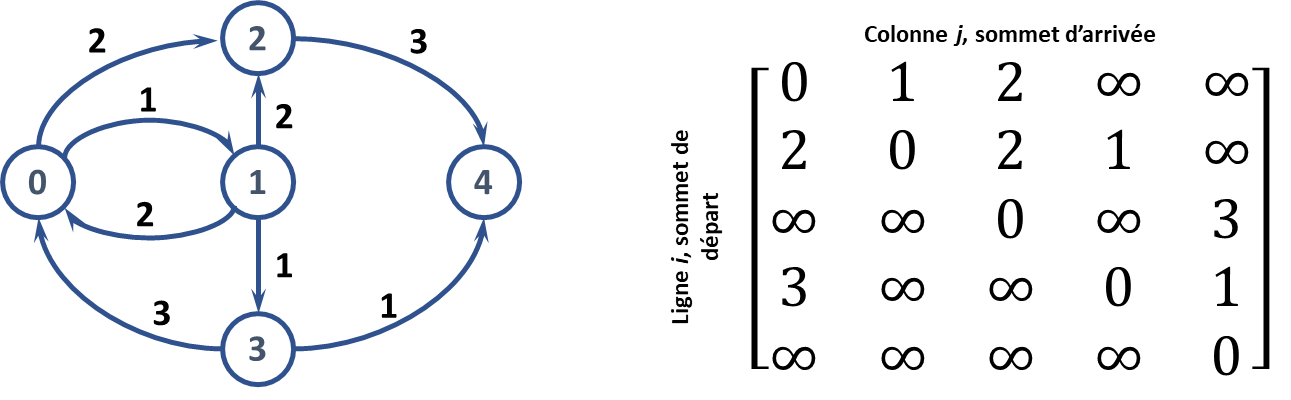
\includegraphics[width=.8\linewidth]{graphe_01}
\end{exemple}